\documentclass[14pt]{extreport}
\usepackage{gost}
%\usepackage{hyperref}
%\usepackage{makecell}
\usepackage{ragged2e}
%\usepackage{graphicx}%Вставка картинок правильная
%\usepackage{float}%"Плавающие" картинки
%\usepackage{wrapfig}%Обтекание фигур (таблиц, картинок и прочего)
%\justifying

\makeatletter
\@addtoreset{figure}{part}% Reset figure numbering at every part
\makeatother
\renewcommand{\thefigure}{\arabic{figure}}% Figure number is part.figure
\renewcommand{\thetable}{\arabic{table}}

%Тут можно вставить дополнительные пакеты

\begin{document}
    \pagestyle{empty} %  выключаем нумерацию
    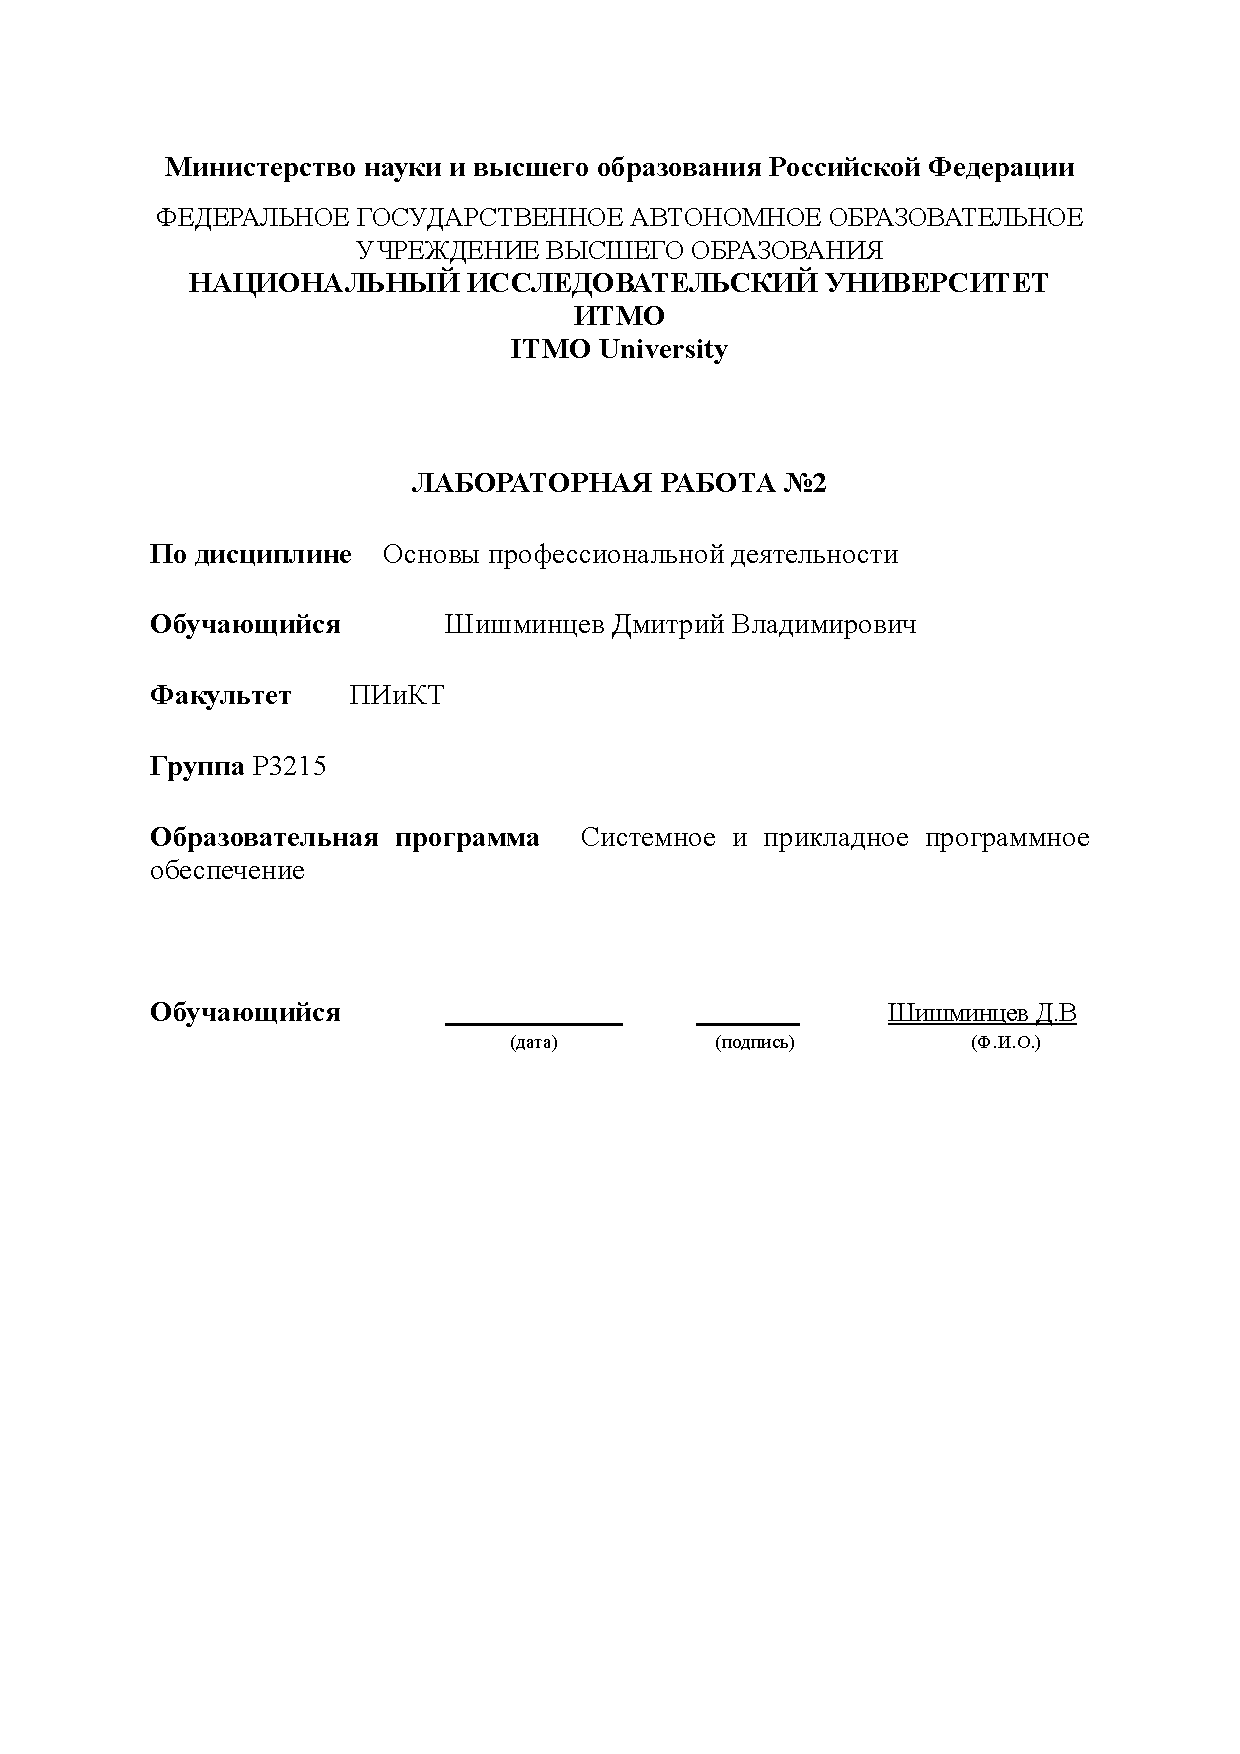
\includepdf[pages=-,pagecommand={}]{title_page.pdf}

    \pagestyle{plain} % включаем нумерацию
    \tableofcontents
    \intro Задание по базовой электронной вычислительной машине (ЭВМ) предполагает анализ программы, определение её функции, области представления и области допустимых значений исходных данных и результатов. В процессе выполнения задания требуется также провести трассировку программы и предложить вариант с уменьшенным числом команд. Этот анализ поможет понять, как программа взаимодействует с данными и как можно оптимизировать её выполнение.

    \chapter{Текст задания}
        По выданному преподавателем варианту восстановить текст заданного варианта программы, определить предназначение и составить описание программы, определить область представления и область допустимых значений исходных данных и результата, выполнить трассировку программы.

        \begin{figure}[!h]
            \centering
            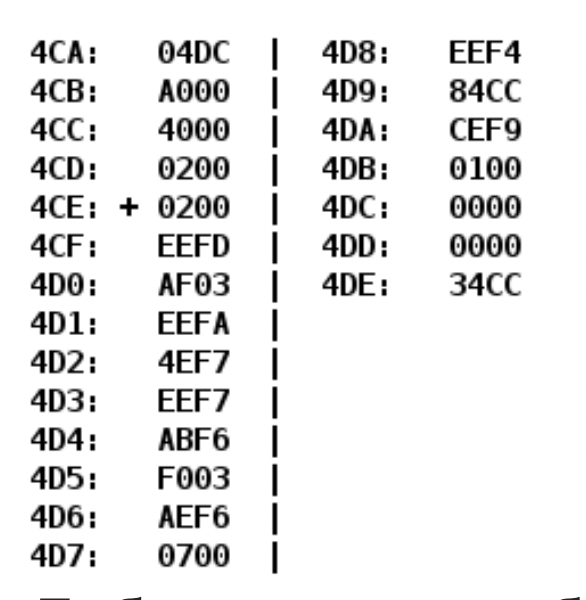
\includegraphics[width=0.4\linewidth]{task.png}
            \caption{Картинка задания}

        \end{figure}


    \chapter{Таблица исходной программы}
        \begin{table}[h]

            \centering
            \begin{tabular}{|c|c|c|c|}
                \hline
                Адрес & Код команды & Мнемоника & Комментарий \\
                \hline
                4CA & 04DC  &  & Указатель на элемент массива\\
                4CB & A000 & & Промежуточная переменная\\
                4CC & 4000 & & Длинна массива\\
                4CD & 0200 & & Счетчик, наш результат\\
                \hline
                \hline
                4CE & 0200 & CLA  & AC = 0 \\
                4CF & EEFD & ST (IP-3)  & [IP-3] = AC \\
                4D0 & AF03 & LD #3  & AC = 3 \\
                4D1 & EEFA & ST (IP-6)  & [IP-6] = AC \\
                4D2 & 4EF7 & ADD (IP-9)  & AC += [IP-9] \\
                4D3 & EEF7 & ST (IP-9)  & [IP-9] = AC \\
                4D4 & ABF6 & LD -(-10)  & AC = [[IP-10]-1] \\
                4D5 & F003 & BEQ 03  & if AC == 0 => JUMP 3 \\
                4D6 & AEF6 & LD (IP-10)  & AC = [IP-10] \\
                4D7 & 0700 & INC  & AC++ \\
                4D8 & EEF4 & ST (IP-12)  & [IP-12] = AC \\
                4D9 & 84CC & LOOP 4CC  & while 4CC >= 0 \\
                4DA & CEF9 & JUMP (IP-7)  & JUMP [IP-7] \\
                4DB & 0100 & HLT  & STOP \\

                \hline
                \hline
                4DC & 0000 & &Элемент массива\\
                4DD & 0000 & &Элемент массива\\
                4DE & 34CC &  & Элемент массива\\
                \hline


            \end{tabular}\label{tab:table}
        \end{table}

    \chapter{Анализ исходной программы}
    \section{Реализуемая функция}
        Программа реализует подсчет ненулевых элементов массива.

    \section{Область допустимых значений}


        Элементы массива: $2^{15} < a[i] < 2^{15}-1$ \\


        Количество элементов массива: $ 0 <= i <= 3$ \\


        Результат: $0 <= r <= i$ \\

    \section{Расположение в памяти ЭВМ}

        Адреса исполняемых команд: 4CE - 4DB

        Адреса исходных данных: 4CA - 4CD, 4DC - 4DE

        \begin{landscape}
            \chapter{Трассировка программы}
            \begin{table}[!h]
                \centering
                \begin{tabular}{|l|l|l|l|l|l|l|l|l|l|l|l|l|}
                    \hline
                    Адр & Знчн & IP & CR & AR & DR & SP & BR & AC & PS & NZVC & Адр & Знчн \\
                    \hline
                    4CB & 04CD & 4CB & 0000 & 000 & 0000 & 000 & 0000 & 0000 & 004 & 0100 &&\\
                    4CB & 04CD & 4CC & 04CD & 4CB & 04CD & 000 & 04CB & 0000 & 004 & 0100 &&\\
                    4CC & 0000 & 4CD & 0000 & 4CC & 0000 & 000 & 04CC & 0000 & 004 & 0100 &&\\
                    4CD & 0003 & 4CE & 0003 & 4CD & 0003 & 000 & 04CD & 0000 & 004 & 0100 &&\\
                    4CE & 0200 & 4CF & 0200 & 4CE & 0200 & 000 & 04CE & 0000 & 004 & 0100 &&\\
                    4CF & EEFD & 4D0 & EEFD & 4CD & 0000 & 000 & FFFD & 0000 & 004 & 0100 & 4CD & 0000 \\
                    4D0 & AF03 & 4D1 & AF03 & 4D0 & 0003 & 000 & 0003 & 0003 & 000 & 0000 &&\\
                    4D1 & EEFA & 4D2 & EEFA & 4CC & 0003 & 000 & FFFA & 0003 & 000 & 0000 & 4CC & 0003 \\
                    4D2 & 4EF7 & 4D3 & 4EF7 & 4CA & 04DC & 000 & FFF7 & 04DF & 000 & 0000 &&\\
                    4D3 & EEF7 & 4D4 & EEF7 & 4CB & 04DF & 000 & FFF7 & 04DF & 000 & 0000 & 4CB & 04DF \\
                    4D4 & ABF6 & 4D5 & ABF6 & 4DE & 34CC & 000 & FFF6 & 34CC & 000 & 0000 & 4CB & 04DE \\
                    4D5 & F003 & 4D6 & F003 & 4D5 & F003 & 000 & 04D5 & 34CC & 000 & 0000 &&\\
                    4D6 & AEF6 & 4D7 & AEF6 & 4CD & 0000 & 000 & FFF6 & 0000 & 004 & 0100 &&\\
                    4D7 & 0700 & 4D8 & 0700 & 4D7 & 0700 & 000 & 04D7 & 0001 & 000 & 0000 &&\\
                    4D8 & EEF4 & 4D9 & EEF4 & 4CD & 0001 & 000 & FFF4 & 0001 & 000 & 0000 & 4CD & 0001 \\
                    4D9 & 84CC & 4DA & 84CC & 4CC & 0002 & 000 & 0001 & 0001 & 000 & 0000 & 4CC & 0002 \\
                    4DA & CEF9 & 4D4 & CEF9 & 4DA & 04D4 & 000 & FFF9 & 0001 & 000 & 0000 &&\\
                    4D4 & ABF6 & 4D5 & ABF6 & 4DD & 0000 & 000 & FFF6 & 0000 & 004 & 0100 & 4CB & 04DD \\
                    4D5 & F003 & 4D9 & F003 & 4D5 & F003 & 000 & 0003 & 0000 & 004 & 0100 &&\\
                    4D9 & 84CC & 4DA & 84CC & 4CC & 0001 & 000 & 0000 & 0000 & 004 & 0100 & 4CC & 0001 \\
                    4DA & CEF9 & 4D4 & CEF9 & 4DA & 04D4 & 000 & FFF9 & 0000 & 004 & 0100 &&\\
                    4D4 & ABF6 & 4D5 & ABF6 & 4DC & 0000 & 000 & FFF6 & 0000 & 004 & 0100 & 4CB & 04DC \\
                    4D5 & F003 & 4D9 & F003 & 4D5 & F003 & 000 & 0003 & 0000 & 004 & 0100 &&\\
                    4D9 & 84CC & 4DB & 84CC & 4CC & 0000 & 000 & FFFF & 0000 & 004 & 0100 & 4CC & 0000 \\
                    4DB & 0100 & 4DC & 0100 & 4DB & 0100 & 000 & 04DB & 0000 & 004 & 0100 &&\\
                    \hline
                \end{tabular}
            \end{table}
        \end{landscape}

    \chapter{Программа на псевдокоде}
        \begin{verbatim}
    4CC = 3 # Длинна массива
    ARRAY[4CC] = [4DE, 4DD, 4DC] # Некий массив из трех элементов
    4CD = 0 # Счетчик
    4CB = 4CA + 3 #  Указатель на элемент массива

    while 4CC >= 0 {
        if [4CB] != 0 {
            4CD++
        }
        4CC--
    }
        \end{verbatim}
    \conclusions Исследование программы на базовой ЭВМ позволяет глубже понять её работу и оптимизировать выполнение, что важно для повышения эффективности и экономии ресурсов. Анализ функции, области представления и области допустимых значений данных, трассировка программы и оптимизация команд помогут более эффективно использовать ресурсы ЭВМ и достичь более эффективных результатов в вычислениях.

\end{document}